% manuscript.tex
% Working manuscript: chest radiograph representation evaluation.
% NOTE: author bylines, author contributions, ethics review/informed consent,
% trial registration, funding, conflict-of-interest disclosures, and submission
% information are intentionally NOT included; none are asserted here and must
% be supplied by the authors.
% Appendix tables use longtable (see back matter); eAppendix is provided by
% \clearpage
\section*{eAppendix. Exploratory 30-Day Acute Readmission After Heart Failure Hospitalization}
\label{sec:readmission-supplement}

\subsection*{Purpose}
We examined whether a frozen chest radiograph representation or image-derived scores for pulmonary edema and cardiomegaly improved discrimination over a structured baseline for 30-day acute readmission after a hospitalization involving heart failure. We separately assessed the feasibility of selecting radiographs closer to discharge and using discharge-window laboratory measurements. This discharge-indexed pilot addressed a different outcome and cohort from the radiograph-indexed ward analysis; it was not a validation of that analysis.

\subsection*{eMethods}
\paragraph{Data and cohort.} We linked the Symile-MIMIC 1.0.0 partition files, metadata, and released radiograph tensors to MIMIC-IV 3.1 hospital data. We included admissions with a heart failure diagnosis and a single Symile-selected frontal radiograph acquired between admission and discharge. Eligible codes were ICD-9-CM 428.x, 398.91, 402.01, 402.11, 402.91, 404.01, 404.03, 404.11, 404.13, 404.91, and 404.93 and ICD-10-CM I50.x, I11.0, I13.0, and I13.2. We retained the original patient-disjoint partitions and, for the retrieval test partition, only the matching positive image for each eligible query. MIMIC-IV-Note 2.2 radiology reports were used only for the separate near-discharge feasibility inventory.

\paragraph{Prediction time and outcome.} Prediction time was discharge. The endpoint was a locally recorded emergency or urgent admission for any cause strictly after discharge and within 30 days. Planned admissions, psychiatric internal transfers, and admissions recorded as transfers from another hospital within 24 hours did not qualify. Death before a qualifying readmission precluded an event; when death was recorded only as a date and a qualifying readmission occurred on the same date, the readmission was counted. Event-free admissions required evidence of follow-up beyond day 30. We excluded index deaths, acute hospital discharges or overlapping admissions, ambiguous returns without a qualifying event, competing deaths, and admissions with insufficient follow-up, including unresolved day-30 death timing. The data did not capture readmissions to other hospitals.

\paragraph{Predictors and fitting.} The structured baseline used age (capped at 91 years), sex, length of stay, admissions in the preceding 30 and 365 days, admission type and source, discharge destination, and AP/PA projection. It did not include discharge laboratory values or vital signs. The global representation used the same frozen NIH-pretrained DenseNet121 pipeline as the ward analysis: a $224\times224$ center crop, conversion to the encoder's single-channel input scale, and global average pooling to 1024 features. The image-only model did not explicitly receive projection metadata. For each finding, a logistic classifier learned from explicit positive and negative report labels; missing or uncertain labels were not treated as negative. Training admissions received out-of-fold scores from patient-disjoint folds, and validation and test scores came from classifiers fit only on labeled training admissions.

\paragraph{Statistical analysis.} For the structured, image-only, and global fusion models, we selected the L2 logistic regression parameter $C$ from 0.0001, 0.001, 0.01, 0.1, and 1 using mean average precision across five stratified patient-grouped training folds (seed 42). Preprocessing parameters were learned within the corresponding fitting partition. For both finding classifiers and score-augmented risk models, we fixed $C=1$ without retuning. The main comparison within the finding-score analysis was the structured model plus both scores vs the structured baseline. We report average precision (AP), area under the receiver operating characteristic curve (AUROC), and paired test differences with percentile 95\% CIs from 2000 patient-level bootstrap resamples. The test partition had been examined previously, and intervals were not adjusted for multiplicity.

\subsection*{eResults}
The analysis included 2439 admissions. The test set included 85 admissions and 13 readmissions (eTable~1). Neither the global embedding nor the finding scores clearly improved on the structured baseline (eTables~2--4). With both scores, the test AP difference was 0.002 (95\% CI, $-0.006$ to 0.011). The AUROC difference was 0.005 (95\% CI, $-0.003$ to 0.014). The image-only model had lower AUROC than the structured baseline in this exploratory split; that contrast does not test performance against chance.

\begingroup
\small
\setlength{\tabcolsep}{4pt}

\noindent\textbf{eTable 1. Cohort flow and 30-day outcome by partition}\par
\begin{longtable}{@{}p{.59\linewidth}rrr@{}}
\toprule
Outcome classification & Train & Validation & Test \\
\midrule
\endhead
Before outcome exclusions & 3488 & 210 & 147 \\
Acute readmission & 617 & 28 & 13 \\
Documented event-free follow-up beyond 30 days & 1623 & 86 & 72 \\
Ambiguous return & 234 & 10 & 9 \\
Competing death within 30 days & 141 & 17 & 9 \\
Unknown follow-up or unresolved death timing & 466 & 39 & 28 \\
Index death & 381 & 27 & 16 \\
Transfer or overlapping admission & 26 & 3 & 0 \\
\midrule
Analysis set, admissions & 2240 & 114 & 85 \\
Analysis set, patients & 1831 & 111 & 84 \\
Readmission rate & 27.5\% & 24.6\% & 15.3\% \\
\bottomrule
\end{longtable}

\noindent\textbf{eTable 2. Coverage of explicit positive and negative report labels}\par
\begin{longtable}{@{}llrrrr@{}}
\toprule
Finding & Partition & Admissions & Labeled & Positive & Negative \\
\midrule
\endhead
Pulmonary edema & Train & 2240 & 1157 & 759 & 398 \\
 & Validation & 114 & 61 & 38 & 23 \\
 & Test & 85 & 39 & 27 & 12 \\
Cardiomegaly & Train & 2240 & 1118 & 1024 & 94 \\
 & Validation & 114 & 72 & 68 & 4 \\
 & Test & 85 & 42 & 40 & 2 \\
\bottomrule
\end{longtable}

\noindent\textbf{eTable 3. Readmission discrimination by model}\par
\begin{longtable}{@{}p{.43\linewidth}rrrr@{}}
\toprule
 & \multicolumn{2}{c}{Validation} & \multicolumn{2}{c}{Test} \\
\cmidrule(lr){2-3}\cmidrule(l){4-5}
Model & AP & AUROC & AP & AUROC \\
\midrule
\endhead
Structured (including AP/PA) & 0.278 & 0.556 & 0.281 & 0.630 \\
Global image embedding only & 0.274 & 0.543 & 0.180 & 0.418 \\
Structured + global embedding & 0.287 & 0.534 & 0.170 & 0.495 \\
Structured + edema score & 0.280 & 0.556 & 0.283 & 0.631 \\
Structured + cardiomegaly score & 0.280 & 0.557 & 0.279 & 0.629 \\
Structured + both scores & 0.279 & 0.553 & 0.283 & 0.636 \\
\bottomrule
\end{longtable}
\noindent The test constant-score reference was AP 0.153 and AUROC 0.500. Selected $C$ values were 1.0 (structured), 0.0001 (image only), and 0.01 (global fusion).
\medskip

\noindent\textbf{eTable 4. Paired test differences from the structured model}\par
\begin{longtable}{@{}p{.32\linewidth}ll@{}}
\toprule
Model & $\Delta$AP (95\% CI) & $\Delta$AUROC (95\% CI) \\
\midrule
\endhead
Global image embedding only & $-0.101$ ($-0.361$ to $0.103$) & $-0.213$ ($-0.416$ to $-0.026$) \\
Structured + global embedding & $-0.110$ ($-0.310$ to $0.003$) & $-0.136$ ($-0.272$ to $0.00002$) \\
Structured + edema score & $0.002$ ($-0.003$ to $0.010$) & $0.001$ ($-0.007$ to $0.009$) \\
Structured + cardiomegaly score & $-0.002$ ($-0.009$ to $0.003$) & $-0.001$ ($-0.007$ to $0.005$) \\
Structured + both scores & $0.002$ ($-0.006$ to $0.011$) & $0.005$ ($-0.003$ to $0.014$) \\
\bottomrule
\end{longtable}
\noindent Extra precision is shown for the global fusion AUROC interval to make clear that its upper bound is positive.
\medskip

\noindent\textbf{eTable 5. Index radiograph timing and projection}\par
\begin{longtable}{@{}lrrrrrrr@{}}
\toprule
Partition & Admissions & $\leq$24 h & $\leq$48 h & $\leq$72 h & $>$72 h & AP view & PA view \\
\midrule
\endhead
Train & 2240 & 145 & 333 & 591 & 1649 & 1920 & 320 \\
Validation & 114 & 10 & 18 & 34 & 80 & 92 & 22 \\
Test & 85 & 6 & 13 & 24 & 61 & 71 & 14 \\
\bottomrule
\end{longtable}
\noindent Timing windows are cumulative, measured backward from discharge. AP view denotes anteroposterior and PA view posteroanterior; elsewhere AP denotes average precision.
\medskip

\noindent\textbf{eTable 6. Near-discharge radiology report inventory}\par
\begin{longtable}{@{}llrrr@{}}
\toprule
Window & Partition & Original image & Report candidate & Difference \\
\midrule
\endhead
24 h & Train & 145 / 143 / 30 & 208 / 203 / 55 & +63 / +60 / +25 \\
 & Validation & 10 / 10 / 2 & 10 / 10 / 1 & 0 / 0 / $-1$ \\
 & Test & 6 / 6 / 0 & 7 / 7 / 1 & +1 / +1 / +1 \\
48 h & Train & 333 / 315 / 74 & 490 / 462 / 155 & +157 / +147 / +81 \\
 & Validation & 18 / 18 / 3 & 21 / 21 / 4 & +3 / +3 / +1 \\
 & Test & 13 / 13 / 1 & 12 / 11 / 1 & $-1$ / $-2$ / 0 \\
72 h & Train & 591 / 550 / 132 & 792 / 723 / 232 & +201 / +173 / +100 \\
 & Validation & 34 / 34 / 6 & 38 / 38 / 8 & +4 / +4 / +2 \\
 & Test & 24 / 24 / 2 & 23 / 22 / 1 & $-1$ / $-2$ / $-1$ \\
\bottomrule
\end{longtable}
\noindent Entries are admissions / patients / readmission events. We selected the in-admission report closest to discharge among same-patient, same-admission reports with frontal projection inferred from text. Across the analysis set, 2086 admissions had at least one report candidate and 1455 had multiple. The candidate set is not a verified superset of the original images. Pixel linkage and corresponding finding labels for newly selected studies were not verified, and no model was fitted to these candidates.
\medskip

\noindent\textbf{eTable 7. Core laboratory and proxy vital-sign coverage before discharge}\par
\begin{longtable}{@{}lrrr@{}}
\toprule
Partition & Admissions & All 5 labs, No. (\%) & All labs and vitals, No. (\%) \\
\midrule
\endhead
Train & 2240 & 2140 (95.5) & 271 (12.1) \\
Validation & 114 & 107 (93.9) & 8 (7.0) \\
Test & 85 & 78 (91.8) & 9 (10.6) \\
\bottomrule
\end{longtable}
\noindent The 48-hour panel comprised creatinine, blood urea nitrogen, sodium, potassium, and bicarbonate. Laboratory values had to be recorded during the admission and stored by discharge. The five vital-sign proxies were heart rate, respiratory rate, systolic blood pressure, oxygen saturation, and temperature from ICU or emergency department data. These proxies do not establish ward vital-sign coverage; emergency department measurement time does not establish independent availability. No test readmissions occurred in the subset with all labs and vitals. No discharge-laboratory or vital-sign model was fitted.

\endgroup

\subsection*{Limitations}
This retrospective, single-center pilot had 13 test events, used a previously examined test partition, and lacked external validation. Event prevalence differed between validation and test, which affects AP. Local outcome ascertainment and exclusion of admissions without documented follow-up constrain generalizability. The finding scores were learned from a partially labeled subset; in particular, only 2 of the 42 test admissions with explicit cardiomegaly labels were labeled negative. Only 13 test radiographs were acquired within 48 hours of discharge, including 1 readmission event, and the report inventory yielded only 1 event at that horizon. The findings therefore do not establish the prognostic value of residual congestion on verified near-discharge radiographs, nor do they establish the value of adding discharge laboratory measurements.
 after the references.
\documentclass[12pt]{article}

\usepackage[margin=1in]{geometry}
\usepackage[T1]{fontenc}
\usepackage{times}
\usepackage{booktabs}
\usepackage{longtable}
\usepackage{array}
\usepackage{xurl}
\usepackage{tikz}
\usetikzlibrary{arrows.meta}
\definecolor{imageblue}{HTML}{24647C}
\definecolor{baselinegray}{HTML}{646D76}

\newcommand{\apaxis}[1]{%
  \draw[baselinegray,densely dashed] (0,0) -- (0,#1);
  \draw[baselinegray] (-.15,0) -- (.45,0);
  \foreach \x/\tick in {-.1/{-0.1},0/0,.1/0.1,.2/0.2,.3/0.3,.4/0.4}
    \draw[baselinegray] (\x,0) -- ++(0,-.10) node[below,text=black] {$\tick$};
  \node[anchor=north] at (.15,-.58) {Difference in average precision};
}
\setlength{\emergencystretch}{1em}

\newcommand{\cit}[1]{\textsuperscript{#1}}

\begin{document}

\begin{center}
{\Large\bfseries What Do Frozen Chest Radiograph Embeddings Add?\par}
\smallskip
{\large Report-Finding Probes and Matched Ablations for 48-Hour Ward Deterioration\par}
\end{center}

\section*{Abstract}

Can a frozen chest radiograph encoder recover findings described in reports, and does its representation improve a downstream prediction once non-image information is available? On separate image-level tasks, adding frozen NIH DenseNet121 embeddings to anteroposterior/posteroanterior projection increased average precision from 0.528 to 0.856 for edema and from 0.669 to 0.884 for pleural effusion; a small balanced pneumothorax probe was inconclusive. We then used 48-hour ICU transfer or in-hospital death as a downstream test on patient-disjoint Symile-MIMIC ward splits. NIH embeddings alone outperformed a constant predictor, but adding them to laboratory results, ECG summaries, and projection changed test average precision by $-0.004$ (paired 95\% CI, $-0.128$ to 0.146). Two image-derived scores for edema and effusion likewise showed no clear gain over laboratories and projection. The reused ward test set contained 26 events, so these comparisons do not rule out a useful gain. The experiments distinguish what can be decoded from a representation from what it adds to a specified downstream baseline.

\section*{Introduction}

A frozen image encoder is useful for transfer when its features preserve information needed by a new task. For chest radiographs, this can mean recovering findings documented in a report or improving a downstream prediction that already uses other inputs. These are distinct tests: a representation can encode a finding without adding information to a downstream model. A comparison with a constant predictor also cannot show whether a model gains information from pixels beyond easily recorded acquisition cues such as radiographic projection.

We used linear probes to test which selected report-derived findings can be decoded from frozen NIH DenseNet121 embeddings beyond anteroposterior (AP) or posteroanterior (PA) projection. We then used 48-hour ward deterioration as a downstream test: on matched admissions, we compared models with and without frozen ImageNet or NIH features under projection-only and structured baselines where applicable. Finally, we tested whether two inspectable, image-derived scores for edema and pleural effusion added information to the same downstream task. This design evaluates existing representations rather than proposing a new encoder or a clinical alert system.

\section*{Methods}

\subsection*{Data Sources, Cohort, and Outcome}

This retrospective secondary analysis used Symile-MIMIC v1.0.0,\cit{3} which links a selected frontal chest radiograph, ECG, and laboratory data for multimodal learning. We used the supplied image selection and the original patient-disjoint splits, not the published Symile objective or weights. The selected image was obtained more than 24 and no more than 72 hours after admission; this was neither a census of ward radiographs nor a cohort indexed to the first emergency department radiograph. For the retrieval test split, only the matched image-admission pair per query was retained; retrieval labels were not used as clinical outcomes.

The unit of analysis was an admission, indexed at acquisition of the selected AP or PA radiograph. MIMIC-IV v3.1 admissions and transfers were used to verify admission identity and ward and ICU timing;\cit{4} admission, discharge, and death times were taken from the Symile master table. We excluded unmatched admissions, images outside the admission, inconsistent death records or death by imaging, ICU entry at or before imaging, and records without a uniquely identifiable general ward at imaging.

The outcome was first ICU transfer or in-hospital death occurring strictly after imaging and no later than the earlier of 48 hours or discharge. ICU transfers were not adjudicated as planned or unplanned. Admissions without an observed event and with insufficient follow-up to determine the outcome were excluded rather than treated as negative.

\subsection*{Structured Predictors}

We used 50 laboratory item--unit combinations selected from training data. For each combination we used the earliest eligible finite value in the 24 hours before or after admission, requiring measurement time to precede or equal recording time and recording time to precede or equal imaging. Results without an admission identifier were eligible only if they belonged to the same patient and were measured before admission within that window. ECG features were 7 waveform summary statistics per lead from 12 leads; the MIMIC-IV-ECG inventory was used to verify patient, record, and acquisition time, and the ECG had to fall within a uniquely identified admission and be acquired no later than imaging.\cit{5} There was no independent timestamp for when ECG results became available. Missing modalities did not result in exclusion. The structured comparator also included AP or PA projection. Concurrent ward vital signs, oxygen use, and mental status needed to reproduce NEWS, NEWS2, MEWS, or qSOFA were not available for a faithful comparison.

\subsection*{Image Representations and Preprocessing}

Both pipelines used the same image tensors and a $224\times224$ center crop. Frozen DenseNet121 encoders produced a 1024-dimensional vector by global average pooling of the final convolutional feature map, without an additional rectified linear activation, classification head, or fine-tuning.\cit{6} The ImageNet pipeline used the normalized 3-channel tensor with TorchVision ImageNet weights.\cit{7} The NIH pipeline reversed the supplied channel normalization, verified that all channels represented the same grayscale image, and mapped the single channel from $[0,1]$ to $[-1024,1024]$ for the TorchXRayVision \texttt{densenet121-res224-nih} encoder.\cit{8} We did not use combined weights trained on MIMIC-CXR. Because preprocessing and weights differed, this comparison estimates the difference between the two pipelines, not the isolated effect of the pretraining dataset.

The main model comparison used the same L2-regularized logistic regression pipeline with laboratories, ECG, and projection, with or without either image embedding. Additional analyses used a constant score equal to training prevalence, image features alone, projection alone, and matched comparisons with smaller structured baselines. We also compared shallow histogram gradient boosting models with laboratories and projection, with or without NIH embeddings; trees had maximum depth 2, learning rate 0.05, at least 30 observations per leaf, and at most 63 bins, with the number of iterations (50 or 100) and L2 penalty (1 or 10) tuned without early stopping.

\subsection*{Image-Level Probes and Image-Derived Scores}

In separate classification analyses, we compared projection alone with projection plus the frozen NIH representation for edema, pleural effusion, and pneumothorax. Image-level samples used the original splits, were deduplicated by examination, and retained only matched retrieval pairs where applicable. We included only explicit positive and negative CheXpert report-derived labels from MIMIC-CXR-JPG; uncertain and blank labels were not considered negative.\cit{9} In a small pneumothorax analysis we sampled an equal number of explicit negative and positive images within each split; AP from this balanced sample does not estimate performance at natural prevalence.

For the ward risk analysis, separate regularized logistic classifiers (C $=$ 0.01) produced scores for edema and pleural effusion from the NIH embeddings. Scores for fitting the risk model were generated out of fold by patient, including within tuning folds; validation and test scores came from image classifiers fitted on training patients only. Report labels were never direct inputs to the risk model. The comparison was laboratories plus projection with vs without the 2 image scores.

\subsection*{Statistical Analysis}

Models used the same patient-grouped 5-fold splits (seed 42) within training. Preprocessing was fitted only on the fitting partition; numeric features were standardized and missing values were mean-imputed with missingness indicators for individual laboratory inputs and for the ECG as a whole when included. For each logistic risk model, C was selected by mean training cross-validation AP from 0.0001, 0.001, 0.01, 0.1, and 1. Final models were fitted on the training split, and the separate validation split was used for checks. The original test split had been evaluated previously; these comparisons are exploratory, not independent validation.

AP summarizes precision over increments in recall and is not the trapezoidal area under the precision-recall curve; for a constant predictor, test AP is the event fraction.\cit{10} We also report AUROC and, for the 3 main matched models, Brier scores. Two-sided percentile 95\% CIs for within-cohort model differences were obtained from 2000 bootstrap resamples by patient, with models compared on the same resamples. No multiplicity adjustment was applied. Differences were computed before rounding.

\section*{Results}

\subsection*{Ward Cohort and Patient-Disjoint Splits}

Filtering within the original splits yielded 3,950 training, 310 validation, and 198 test admissions (Fig.~\ref{fig:cohort}). The test split contained 26 events. At least one eligible laboratory result was available for 3,916, 306, and 197 admissions across the three splits; a time-matched ECG was available for 921, 78, and 51, respectively.

\begin{figure}[htbp]
\centering
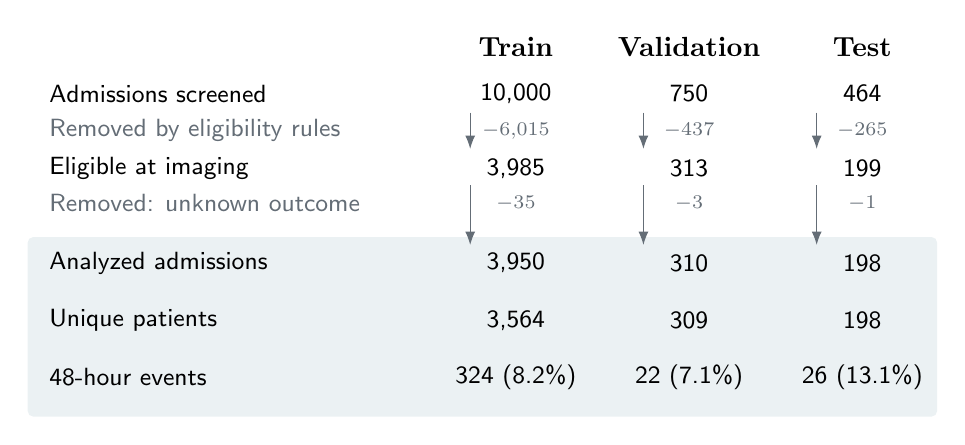
\begin{tikzpicture}[x=1cm,y=1cm,font=\small\sffamily,>=Latex]
  \foreach \x/\heading in {6.2/Train,8.4/Validation,10.6/Test}
    \node[font=\bfseries] at (\x,0) {\heading};
  \fill[imageblue!9,rounded corners=2pt] (0,-4.7) rectangle (11.55,-2.42);
  \foreach \y/\label/\train/\val/\test in {
    -.60/Admissions screened/{10,000}/750/464,
    -1.55/Eligible at imaging/{3,985}/313/199,
    -2.75/Analyzed admissions/{3,950}/310/198,
    -3.48/Unique patients/{3,564}/309/198,
    -4.20/{48-hour events}/324 (8.2\%)/22 (7.1\%)/26 (13.1\%)} {
      \node[anchor=west] at (.15,\y) {\label};
      \node at (6.2,\y) {\train};
      \node at (8.4,\y) {\val};
      \node at (10.6,\y) {\test};
  }
  \foreach \x in {5.62,7.82,10.02} {
    \draw[->,baselinegray] (\x,-.84) -- (\x,-1.30);
    \draw[->,baselinegray] (\x,-1.76) -- (\x,-2.52);
  }
  \node[anchor=west,text=baselinegray] at (.15,-1.07) {Removed by eligibility rules};
  \node[anchor=west,text=baselinegray] at (.15,-1.99) {Removed: unknown outcome};
  \foreach \x/\elig/\unknown in {6.2/{6,015}/35,8.4/437/3,10.6/265/1} {
    \node[font=\scriptsize,text=baselinegray,fill=white,inner sep=1pt] at (\x,-1.07) {$-$\elig};
    \node[font=\scriptsize,text=baselinegray] at (\x,-1.99) {$-$\unknown};
  }
\end{tikzpicture}
\caption{Ward cohort flow. Screening began after unmatched retrieval candidates were removed. Eligibility and outcome ascertainment were applied within the original Symile-MIMIC patient-disjoint splits; no patients were reassigned. Event percentages use analyzed admissions as denominators.}
\label{fig:cohort}
\end{figure}

\subsection*{Edema and Pleural Effusion Are Decodable Beyond Projection}

Adding NIH embeddings to projection improved average precision (AP) for report-derived edema and pleural effusion; the small, balanced pneumothorax probe was inconclusive (Fig.~\ref{fig:probe}; Table~\ref{tab:probe}). These image-level comparisons show which selected labels the linear probes could recover, not where in the image the evidence lay. When the two corresponding image-derived scores were added to the ward model with laboratories and projection, AP changed from 0.244 to 0.239, with a confidence interval spanning both a decrease and an increase (Fig.~\ref{fig:probe}; Table~\ref{tab:sens}).

\begin{figure}[htbp]
\centering
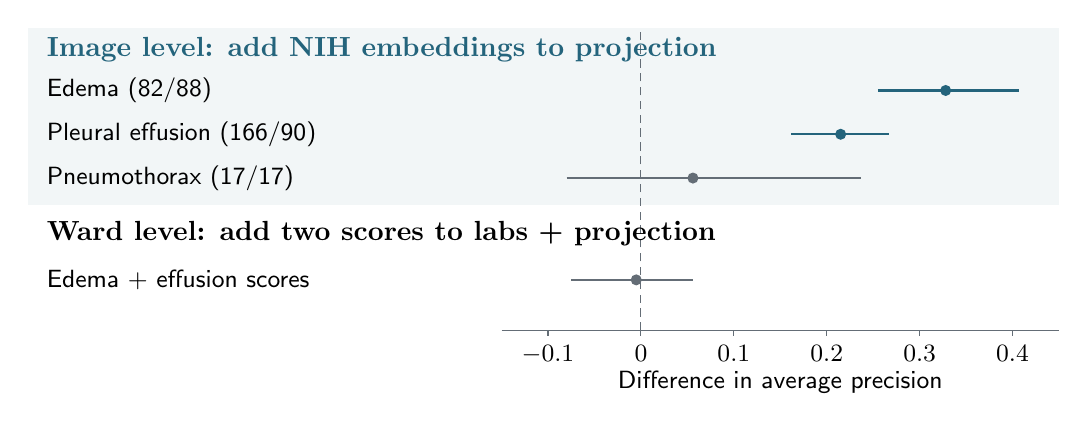
\begin{tikzpicture}[x=11.8cm,y=.67cm,font=\small\sffamily]
  \fill[imageblue!6] (-.66,2.37) rectangle (.45,5.73);
  \apaxis{5.73}
  \node[anchor=west,font=\bfseries,text=imageblue] at (-.65,5.33) {Image level: add NIH embeddings to projection};
  \node[anchor=west,font=\bfseries] at (-.65,1.83) {Ward level: add two scores to labs + projection};
  \foreach \y/\label/\point/\lo/\hi/\ink in {
    4.55/{Edema (82/88)}/.328/.255/.407/imageblue,
    3.72/{Pleural effusion (166/90)}/.215/.162/.267/imageblue,
    2.89/{Pneumothorax (17/17)}/.056/-.080/.237/baselinegray,
    .96/{Edema + effusion scores}/-.005/-.075/.056/baselinegray} {
      \node[anchor=west] at (-.65,\y) {\label};
      \draw[\ink,thick] (\lo,\y) -- (\hi,\y);
      \fill[\ink] (\point,\y) circle[radius=2pt];
  }
\end{tikzpicture}
\caption{Finding probes and the downstream score test. Dots show the augmented model's test AP minus the baseline's; bars show paired patient-bootstrap 95\% confidence intervals. Image rows show positive/negative image counts for each separate report-label test set. The pneumothorax sample was balanced; its absolute AP does not estimate performance at natural prevalence. The last row tests two image-derived scores on the separate ward test set (198 admissions, 26 events), not the full embedding.}
\label{fig:probe}
\end{figure}

\subsection*{The Incremental Ward Result Depends on the Baseline}

NIH embeddings alone outperformed a constant predictor (AP, 0.234 vs 0.131), but when projection was the comparator, the AP difference was 0.058 (95\% CI, $-0.009$ to 0.215). With laboratories, ECG, and projection already included, neither pipeline showed a clear gain (Fig.~\ref{fig:ward}; Table~\ref{tab:main}). NIH had the higher point estimates of the two image pipelines on test, but the ranking reversed on validation; the test AP difference was 0.019 (95\% CI, $-0.066$ to 0.150).

The sensitivity analyses did not settle whether a different baseline or model could benefit. Adding NIH features to laboratories without projection yielded a positive point estimate, whereas including projection in the logistic baseline removed that apparent gain. A shallow tree comparison with laboratories and projection also yielded a positive but imprecise estimate (AP difference, 0.095; 95\% CI, $-0.057$ to 0.255; Table~\ref{tab:sens}).

\begin{figure}[htbp]
\centering
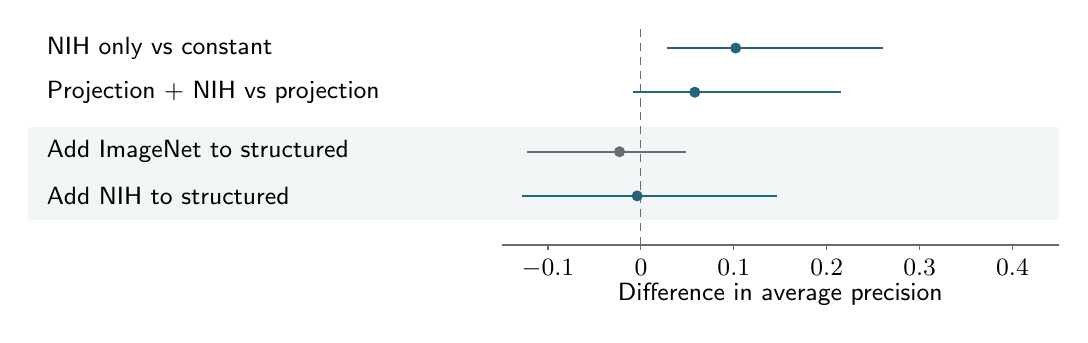
\begin{tikzpicture}[x=11.8cm,y=.63cm,font=\small\sffamily]
  \fill[imageblue!6] (-.66,.51) rectangle (.45,2.38);
  \apaxis{4.37}
  \foreach \y/\label/\point/\lo/\hi/\ink in {
    3.97/{NIH only vs constant}/.102/.028/.261/imageblue,
    3.08/{Projection + NIH vs projection}/.058/-.009/.215/imageblue,
    1.88/{Add ImageNet to structured}/-.023/-.123/.048/baselinegray,
    .99/{Add NIH to structured}/-.004/-.128/.146/imageblue} {
      \node[anchor=west] at (-.65,\y) {\label};
      \draw[\ink,thick] (\lo,\y) -- (\hi,\y);
      \fill[\ink] (\point,\y) circle[radius=2pt];
  }
\end{tikzpicture}
\caption{Matched ward ablations on 198 test admissions (26 events). Dots show test AP differences (image model minus the stated baseline); bars show paired patient-bootstrap 95\% confidence intervals. The structured baseline includes laboratories, ECG and AP/PA projection. All rows evaluate the same admissions.}
\label{fig:ward}
\end{figure}

\subsection*{Exploratory Heart Failure Readmission Pilot}

A separate exploratory pilot evaluated 30-day acute readmission after discharge among admissions with heart failure. Its endpoint, prediction time, and eligible cohort differed from those of the ward analysis; results are reported in the eAppendix and are not a validation of the ward model.

\section*{Discussion}

A finding can be readily decoded from a frozen representation without yielding a measurable improvement on a different task. Here the probes test whether the embedding carries information about selected report labels beyond projection. The two-score ablation asks whether a model benefits from adding those particular image-derived summaries. Neither experiment localizes features, attributes individual risk predictions, or tests whether the findings mediate any effect of the full embedding. A null or imprecise two-score result does not show that the full embedding ignores those findings.

Projection is an informative baseline because it may reflect acquisition circumstances or patient status. Its performance does not prove that the encoder relies on projection, but it makes a comparison against a constant alone insufficient to establish what pixels add. Earlier exploratory neural fusion models on the same test set also showed weak discrimination; these runs are not independent confirmation. The available estimates do not establish equivalence or rule out gains for other encoders, downstream models, or baselines.

The imaging-indexed task is not directly comparable with repeated ward early warning measurements or disease-specific emergency department imaging studies.\cit{1,2} A next representation benchmark could prespecify the projection and multimodal controls, pair images with measurements taken near acquisition, and use a fresh test set large enough to distinguish a practically meaningful AP gain from noise. A separate evaluation with spatial annotations would be needed to test localization.

\subsection*{Limitations}

The selected Symile radiographs represent a subset of admissions imaged within a restricted time window; results do not generalize directly to all ward admissions or to emergency department triage. Some ICU transfers may have been planned, and discharge ends ascertainment of the in-hospital outcome. Structured inputs were sparse for ECG (51 of 198 test admissions), laboratory results did not necessarily describe the state immediately before imaging, and a faithful bedside early warning comparator could not be constructed: a proxy count based on emergency department recorded measurement times found respiratory rate and oxygen saturation jointly recorded for only 49, 3, and 2 admissions in the training, validation, and test splits, which does not establish the availability of contemporaneous general-ward vital signs; oxygen therapy and mental status were not verifiable, and proxy scoring was not attempted. Image-level reference standards were report-derived, not independently adjudicated, and performance on those labels does not establish radiologist-level diagnosis or explain the model's risk predictions. The head-to-head encoder comparison does not isolate pretraining effects. The test set was reused and included 26 events; intervals were wide, analyses were not multiplicity adjusted, and no external or prospective performance or clinical utility was assessed.

\section*{Conclusions}

Frozen chest radiograph embeddings improved recognition of selected report-derived findings and contained standalone prognostic signal for 48-hour ICU transfer or death. Their incremental value over available structured variables at the time of imaging was not established.

\section*{References}

\begin{enumerate}
\item Edelson DP, Churpek MM, Carey KA, et al. Early warning scores with and without artificial intelligence. \textit{JAMA Netw Open}. 2024;7(10):e2438986. \url{doi:10.1001/jamanetworkopen.2024.38986}
\item Shamout FE, Shen Y, Wu N, et al. An artificial intelligence system for predicting the deterioration of COVID-19 patients in the emergency department. \textit{NPJ Digit Med}. 2021;4:80. \url{doi:10.1038/s41746-021-00453-0}
\item Saporta A, Puli AM, Goldstein M, Ranganath R. Symile-MIMIC: a multimodal clinical dataset of chest X-rays, electrocardiograms, and blood labs from MIMIC-IV. Version 1.0.0. PhysioNet; 2025. \url{doi:10.13026/3vvj-s428}
\item Johnson A, Bulgarelli L, Pollard T, et al. MIMIC-IV. Version 3.1. PhysioNet; 2024. \url{doi:10.13026/kpb9-mt58}
\item Gow B, Pollard T, Nathanson LA, et al. MIMIC-IV-ECG: Diagnostic Electrocardiogram Matched Subset. Version 1.0. PhysioNet; 2023. \url{doi:10.13026/4nqg-sb35}
\item Huang G, Liu Z, Van Der Maaten L, Weinberger KQ. Densely connected convolutional networks. In: \textit{Proceedings of the IEEE Conference on Computer Vision and Pattern Recognition}; 2017.
\item TorchVision. DenseNet121 model documentation: \url{DenseNet121_Weights.IMAGENET1K_V1}. \url{https://docs.pytorch.org/vision/stable/models/generated/torchvision.models.densenet121.html}
\item TorchXRayVision. DenseNet121 model definitions and NIH-specific \url{densenet121-res224-nih} checkpoint. \url{https://github.com/mlmed/torchxrayvision/blob/master/torchxrayvision/models.py}
\item Johnson A, Lungren M, Peng Y, et al. MIMIC-CXR-JPG: chest radiographs with structured labels. Version 2.0.0. PhysioNet; 2019. \url{doi:10.13026/8360-t248}
\item Saito T, Rehmsmeier M. The precision-recall plot is more informative than the ROC plot when evaluating binary classifiers on imbalanced datasets. \textit{PLoS One}. 2015;10(3):\allowbreak e0118432. \url{doi:10.1371/journal.pone.0118432}
\end{enumerate}

% ---------------- Back matter: tables (longtable) ----------------

{\footnotesize
\setlength{\tabcolsep}{3pt}
\begin{longtable}{@{}p{4.3cm}ccp{2.2cm}p{2.7cm}p{2.7cm}@{}}
\caption{Test Performance for 48-Hour ICU Transfer or In-Hospital Death}\label{tab:main}\\
\toprule
Model & AP & AUROC & Comparator for difference & AP difference (95\% CI) & AUROC difference (95\% CI) \\
\midrule
\endfirsthead
\caption[]{Test Performance for 48-Hour ICU Transfer or In-Hospital Death (continued)}\\
\toprule
Model & AP & AUROC & Comparator for difference & AP difference (95\% CI) & AUROC difference (95\% CI) \\
\midrule
\endhead
\bottomrule
\endlastfoot
Constant score & 0.131 & 0.500 & --- & --- & --- \\
NIH embeddings only & 0.234 & 0.659 & Constant score & 0.102 (0.028 to 0.261) & 0.159 (0.047 to 0.260) \\
Projection only & 0.176 & 0.644 & --- & --- & --- \\
Laboratories + ECG + projection & 0.234 & 0.662 & --- & --- & --- \\
\quad + ImageNet embeddings & 0.211 & 0.653 & Laboratories + ECG + projection & $-0.023$ ($-0.123$ to 0.048) & $-0.009$ ($-0.115$ to 0.101) \\
\quad + NIH embeddings & 0.230 & 0.672 & Laboratories + ECG + projection & $-0.004$ ($-0.128$ to 0.146) & 0.009 ($-0.097$ to 0.122) \\
\end{longtable}
\par\noindent{\footnotesize All rows use the same 198 test admissions (26 events). AP indicates average precision; AUROC, area under the receiver operating characteristic curve; CI, confidence interval; ECG, electrocardiogram; NIH, National Institutes of Health. Differences are paired by patient (2000 bootstrap resamples). Selected C values: 0.01 (structured), 0.001 (with ImageNet embeddings), 0.001 (with NIH embeddings). Test Brier scores were 0.112 (structured), 0.114 (with ImageNet embeddings), and 0.113 (with NIH embeddings).\par}
}

\bigskip

{\footnotesize
\setlength{\tabcolsep}{3pt}
\begin{longtable}{@{}p{3.6cm}p{2.7cm}p{2.7cm}p{3.1cm}p{3.1cm}@{}}
\caption{Test Performance for Classification of Report-Derived Findings}\label{tab:probe}\\
\toprule
Finding (positive/negative images) & AP: projection / + NIH & AUROC: projection / + NIH & AP difference (95\% CI) & AUROC difference (95\% CI) \\
\midrule
\endfirsthead
\caption[]{Test Performance for Classification of Report-Derived Findings (continued)}\\
\toprule
Finding (positive/negative images) & AP: projection / + NIH & AUROC: projection / + NIH & AP difference (95\% CI) & AUROC difference (95\% CI) \\
\midrule
\endhead
\bottomrule
\endlastfoot
Edema (82/88) & 0.528 / 0.856 & 0.583 / 0.861 & 0.328 (0.255 to 0.407) & 0.278 (0.209 to 0.342) \\
Pleural effusion (166/90) & 0.669 / 0.884 & 0.543 / 0.814 & 0.215 (0.162 to 0.267) & 0.271 (0.201 to 0.334) \\
Pneumothorax (17/17; balanced sample) & 0.518 / 0.574 & 0.529 / 0.574 & 0.056 ($-0.080$ to 0.237) & 0.045 ($-0.161$ to 0.242) \\
\end{longtable}
\par\noindent{\footnotesize Samples differ by finding and are not the 198-admission prognosis test set. Differences compare projection plus NIH embeddings with projection alone on the same images for each finding. The pneumothorax sample was balanced within each split (17 positive and 17 negative test images); AP on this balanced sample does not estimate performance at natural prevalence. CI indicates confidence interval; NIH, National Institutes of Health.\par}
}

\bigskip

{\footnotesize
\setlength{\tabcolsep}{3pt}
\begin{longtable}{@{}p{4.2cm}p{2.4cm}p{2.4cm}p{3.0cm}p{3.0cm}@{}}
\caption{Sensitivity and Control Analyses for 48-Hour ICU Transfer or In-Hospital Death}\label{tab:sens}\\
\toprule
Comparison (baseline $\rightarrow$ augmented) & Validation AP / AUROC & Test AP / AUROC & Test AP difference (95\% CI) & Test AUROC difference (95\% CI) \\
\midrule
\endfirsthead
\caption[]{Sensitivity and Control Analyses for 48-Hour ICU Transfer or In-Hospital Death (continued)}\\
\toprule
Comparison (baseline $\rightarrow$ augmented) & Validation AP / AUROC & Test AP / AUROC & Test AP difference (95\% CI) & Test AUROC difference (95\% CI) \\
\midrule
\endhead
\bottomrule
\endlastfoot
Projection only $\rightarrow$ projection + NIH (logistic regression) & --- & 0.176 / 0.644 $\rightarrow$ 0.234 / 0.659 & 0.058 ($-0.009$ to 0.215) & 0.016 ($-0.080$ to 0.107) \\
Laboratories only $\rightarrow$ laboratories + NIH (logistic regression) & 0.140 / 0.584 $\rightarrow$ 0.142 / 0.648 & 0.185 / 0.584 $\rightarrow$ 0.245 / 0.672 & 0.060 ($-0.041$ to 0.197) & 0.088 ($-0.039$ to 0.221) \\
Laboratories + projection $\rightarrow$ + NIH (logistic regression) & 0.131 / 0.630 $\rightarrow$ 0.140 / 0.650 & 0.244 / 0.679 $\rightarrow$ 0.240 / 0.676 & $-0.004$ (CI not reported) & $-0.003$ (CI not reported) \\
Laboratories + projection $\rightarrow$ + edema and effusion scores (logistic regression) & 0.131 / 0.630 $\rightarrow$ 0.141 / 0.645 & 0.244 / 0.679 $\rightarrow$ 0.239 / 0.678 & $-0.005$ ($-0.075$ to 0.056) & $-0.001$ ($-0.074$ to 0.074) \\
Laboratories + projection $\rightarrow$ + NIH (shallow gradient boosting) & 0.130 / 0.645 $\rightarrow$ 0.159 / 0.645 & 0.178 / 0.587 $\rightarrow$ 0.274 / 0.651 & 0.095 ($-0.057$ to 0.255) & 0.064 ($-0.053$ to 0.176) \\
\end{longtable}
\par\noindent{\footnotesize Each row compares the same model family before and after adding features. Differences are paired by patient (2000 bootstrap resamples) on the 198-admission test set. Shallow gradient boosting trees: maximum depth 2, learning rate 0.05, minimum 30 observations per leaf, at most 63 bins; 50 iterations and L2 penalty of 1 were selected within training for both tree models. AP indicates average precision; AUROC, area under the receiver operating characteristic curve; CI, confidence interval; NIH, National Institutes of Health.\par}
}

% ---------------- eAppendix (provided by collaborator; do not edit) ----------------
\clearpage
\section*{eAppendix. Exploratory 30-Day Acute Readmission After Heart Failure Hospitalization}
\label{sec:readmission-supplement}

\subsection*{Purpose}
We examined whether a frozen chest radiograph representation or image-derived scores for pulmonary edema and cardiomegaly improved discrimination over a structured baseline for 30-day acute readmission after a hospitalization involving heart failure. We separately assessed the feasibility of selecting radiographs closer to discharge and using discharge-window laboratory measurements. This discharge-indexed pilot addressed a different outcome and cohort from the radiograph-indexed ward analysis; it was not a validation of that analysis.

\subsection*{eMethods}
\paragraph{Data and cohort.} We linked the Symile-MIMIC 1.0.0 partition files, metadata, and released radiograph tensors to MIMIC-IV 3.1 hospital data. We included admissions with a heart failure diagnosis and a single Symile-selected frontal radiograph acquired between admission and discharge. Eligible codes were ICD-9-CM 428.x, 398.91, 402.01, 402.11, 402.91, 404.01, 404.03, 404.11, 404.13, 404.91, and 404.93 and ICD-10-CM I50.x, I11.0, I13.0, and I13.2. We retained the original patient-disjoint partitions and, for the retrieval test partition, only the matching positive image for each eligible query. MIMIC-IV-Note 2.2 radiology reports were used only for the separate near-discharge feasibility inventory.

\paragraph{Prediction time and outcome.} Prediction time was discharge. The endpoint was a locally recorded emergency or urgent admission for any cause strictly after discharge and within 30 days. Planned admissions, psychiatric internal transfers, and admissions recorded as transfers from another hospital within 24 hours did not qualify. Death before a qualifying readmission precluded an event; when death was recorded only as a date and a qualifying readmission occurred on the same date, the readmission was counted. Event-free admissions required evidence of follow-up beyond day 30. We excluded index deaths, acute hospital discharges or overlapping admissions, ambiguous returns without a qualifying event, competing deaths, and admissions with insufficient follow-up, including unresolved day-30 death timing. The data did not capture readmissions to other hospitals.

\paragraph{Predictors and fitting.} The structured baseline used age (capped at 91 years), sex, length of stay, admissions in the preceding 30 and 365 days, admission type and source, discharge destination, and AP/PA projection. It did not include discharge laboratory values or vital signs. The global representation used the same frozen NIH-pretrained DenseNet121 pipeline as the ward analysis: a $224\times224$ center crop, conversion to the encoder's single-channel input scale, and global average pooling to 1024 features. The image-only model did not explicitly receive projection metadata. For each finding, a logistic classifier learned from explicit positive and negative report labels; missing or uncertain labels were not treated as negative. Training admissions received out-of-fold scores from patient-disjoint folds, and validation and test scores came from classifiers fit only on labeled training admissions.

\paragraph{Statistical analysis.} For the structured, image-only, and global fusion models, we selected the L2 logistic regression parameter $C$ from 0.0001, 0.001, 0.01, 0.1, and 1 using mean average precision across five stratified patient-grouped training folds (seed 42). Preprocessing parameters were learned within the corresponding fitting partition. For both finding classifiers and score-augmented risk models, we fixed $C=1$ without retuning. The main comparison within the finding-score analysis was the structured model plus both scores vs the structured baseline. We report average precision (AP), area under the receiver operating characteristic curve (AUROC), and paired test differences with percentile 95\% CIs from 2000 patient-level bootstrap resamples. The test partition had been examined previously, and intervals were not adjusted for multiplicity.

\subsection*{eResults}
The analysis included 2439 admissions. The test set included 85 admissions and 13 readmissions (eTable~1). Neither the global embedding nor the finding scores clearly improved on the structured baseline (eTables~2--4). With both scores, the test AP difference was 0.002 (95\% CI, $-0.006$ to 0.011). The AUROC difference was 0.005 (95\% CI, $-0.003$ to 0.014). The image-only model had lower AUROC than the structured baseline in this exploratory split; that contrast does not test performance against chance.

\begingroup
\small
\setlength{\tabcolsep}{4pt}

\noindent\textbf{eTable 1. Cohort flow and 30-day outcome by partition}\par
\begin{longtable}{@{}p{.59\linewidth}rrr@{}}
\toprule
Outcome classification & Train & Validation & Test \\
\midrule
\endhead
Before outcome exclusions & 3488 & 210 & 147 \\
Acute readmission & 617 & 28 & 13 \\
Documented event-free follow-up beyond 30 days & 1623 & 86 & 72 \\
Ambiguous return & 234 & 10 & 9 \\
Competing death within 30 days & 141 & 17 & 9 \\
Unknown follow-up or unresolved death timing & 466 & 39 & 28 \\
Index death & 381 & 27 & 16 \\
Transfer or overlapping admission & 26 & 3 & 0 \\
\midrule
Analysis set, admissions & 2240 & 114 & 85 \\
Analysis set, patients & 1831 & 111 & 84 \\
Readmission rate & 27.5\% & 24.6\% & 15.3\% \\
\bottomrule
\end{longtable}

\noindent\textbf{eTable 2. Coverage of explicit positive and negative report labels}\par
\begin{longtable}{@{}llrrrr@{}}
\toprule
Finding & Partition & Admissions & Labeled & Positive & Negative \\
\midrule
\endhead
Pulmonary edema & Train & 2240 & 1157 & 759 & 398 \\
 & Validation & 114 & 61 & 38 & 23 \\
 & Test & 85 & 39 & 27 & 12 \\
Cardiomegaly & Train & 2240 & 1118 & 1024 & 94 \\
 & Validation & 114 & 72 & 68 & 4 \\
 & Test & 85 & 42 & 40 & 2 \\
\bottomrule
\end{longtable}

\noindent\textbf{eTable 3. Readmission discrimination by model}\par
\begin{longtable}{@{}p{.43\linewidth}rrrr@{}}
\toprule
 & \multicolumn{2}{c}{Validation} & \multicolumn{2}{c}{Test} \\
\cmidrule(lr){2-3}\cmidrule(l){4-5}
Model & AP & AUROC & AP & AUROC \\
\midrule
\endhead
Structured (including AP/PA) & 0.278 & 0.556 & 0.281 & 0.630 \\
Global image embedding only & 0.274 & 0.543 & 0.180 & 0.418 \\
Structured + global embedding & 0.287 & 0.534 & 0.170 & 0.495 \\
Structured + edema score & 0.280 & 0.556 & 0.283 & 0.631 \\
Structured + cardiomegaly score & 0.280 & 0.557 & 0.279 & 0.629 \\
Structured + both scores & 0.279 & 0.553 & 0.283 & 0.636 \\
\bottomrule
\end{longtable}
\noindent The test constant-score reference was AP 0.153 and AUROC 0.500. Selected $C$ values were 1.0 (structured), 0.0001 (image only), and 0.01 (global fusion).
\medskip

\noindent\textbf{eTable 4. Paired test differences from the structured model}\par
\begin{longtable}{@{}p{.32\linewidth}ll@{}}
\toprule
Model & $\Delta$AP (95\% CI) & $\Delta$AUROC (95\% CI) \\
\midrule
\endhead
Global image embedding only & $-0.101$ ($-0.361$ to $0.103$) & $-0.213$ ($-0.416$ to $-0.026$) \\
Structured + global embedding & $-0.110$ ($-0.310$ to $0.003$) & $-0.136$ ($-0.272$ to $0.00002$) \\
Structured + edema score & $0.002$ ($-0.003$ to $0.010$) & $0.001$ ($-0.007$ to $0.009$) \\
Structured + cardiomegaly score & $-0.002$ ($-0.009$ to $0.003$) & $-0.001$ ($-0.007$ to $0.005$) \\
Structured + both scores & $0.002$ ($-0.006$ to $0.011$) & $0.005$ ($-0.003$ to $0.014$) \\
\bottomrule
\end{longtable}
\noindent Extra precision is shown for the global fusion AUROC interval to make clear that its upper bound is positive.
\medskip

\noindent\textbf{eTable 5. Index radiograph timing and projection}\par
\begin{longtable}{@{}lrrrrrrr@{}}
\toprule
Partition & Admissions & $\leq$24 h & $\leq$48 h & $\leq$72 h & $>$72 h & AP view & PA view \\
\midrule
\endhead
Train & 2240 & 145 & 333 & 591 & 1649 & 1920 & 320 \\
Validation & 114 & 10 & 18 & 34 & 80 & 92 & 22 \\
Test & 85 & 6 & 13 & 24 & 61 & 71 & 14 \\
\bottomrule
\end{longtable}
\noindent Timing windows are cumulative, measured backward from discharge. AP view denotes anteroposterior and PA view posteroanterior; elsewhere AP denotes average precision.
\medskip

\noindent\textbf{eTable 6. Near-discharge radiology report inventory}\par
\begin{longtable}{@{}llrrr@{}}
\toprule
Window & Partition & Original image & Report candidate & Difference \\
\midrule
\endhead
24 h & Train & 145 / 143 / 30 & 208 / 203 / 55 & +63 / +60 / +25 \\
 & Validation & 10 / 10 / 2 & 10 / 10 / 1 & 0 / 0 / $-1$ \\
 & Test & 6 / 6 / 0 & 7 / 7 / 1 & +1 / +1 / +1 \\
48 h & Train & 333 / 315 / 74 & 490 / 462 / 155 & +157 / +147 / +81 \\
 & Validation & 18 / 18 / 3 & 21 / 21 / 4 & +3 / +3 / +1 \\
 & Test & 13 / 13 / 1 & 12 / 11 / 1 & $-1$ / $-2$ / 0 \\
72 h & Train & 591 / 550 / 132 & 792 / 723 / 232 & +201 / +173 / +100 \\
 & Validation & 34 / 34 / 6 & 38 / 38 / 8 & +4 / +4 / +2 \\
 & Test & 24 / 24 / 2 & 23 / 22 / 1 & $-1$ / $-2$ / $-1$ \\
\bottomrule
\end{longtable}
\noindent Entries are admissions / patients / readmission events. We selected the in-admission report closest to discharge among same-patient, same-admission reports with frontal projection inferred from text. Across the analysis set, 2086 admissions had at least one report candidate and 1455 had multiple. The candidate set is not a verified superset of the original images. Pixel linkage and corresponding finding labels for newly selected studies were not verified, and no model was fitted to these candidates.
\medskip

\noindent\textbf{eTable 7. Core laboratory and proxy vital-sign coverage before discharge}\par
\begin{longtable}{@{}lrrr@{}}
\toprule
Partition & Admissions & All 5 labs, No. (\%) & All labs and vitals, No. (\%) \\
\midrule
\endhead
Train & 2240 & 2140 (95.5) & 271 (12.1) \\
Validation & 114 & 107 (93.9) & 8 (7.0) \\
Test & 85 & 78 (91.8) & 9 (10.6) \\
\bottomrule
\end{longtable}
\noindent The 48-hour panel comprised creatinine, blood urea nitrogen, sodium, potassium, and bicarbonate. Laboratory values had to be recorded during the admission and stored by discharge. The five vital-sign proxies were heart rate, respiratory rate, systolic blood pressure, oxygen saturation, and temperature from ICU or emergency department data. These proxies do not establish ward vital-sign coverage; emergency department measurement time does not establish independent availability. No test readmissions occurred in the subset with all labs and vitals. No discharge-laboratory or vital-sign model was fitted.

\endgroup

\subsection*{Limitations}
This retrospective, single-center pilot had 13 test events, used a previously examined test partition, and lacked external validation. Event prevalence differed between validation and test, which affects AP. Local outcome ascertainment and exclusion of admissions without documented follow-up constrain generalizability. The finding scores were learned from a partially labeled subset; in particular, only 2 of the 42 test admissions with explicit cardiomegaly labels were labeled negative. Only 13 test radiographs were acquired within 48 hours of discharge, including 1 readmission event, and the report inventory yielded only 1 event at that horizon. The findings therefore do not establish the prognostic value of residual congestion on verified near-discharge radiographs, nor do they establish the value of adding discharge laboratory measurements.


\end{document}
